\section{Entropy and Temperature}

\makelabheader %(Space for student name, etc., defined in master.tex)

\textbf{Objective}

To explore the connection between the fundamental definition of entropy and
temperature.

\textbf{Overview}

Consider the microscopic  definition of the entropy of a system
\begin{equation}
S = k_B \ln \Omega
\end{equation}
where $k_B$ is Boltzmann's constant and $\Omega$ is the multiplicity or number of 
microstates.
A microstate is defined by a particular arrangement of energy quanta among the
atoms.
A macrostate is defined by the total number of energy quanta $q$ and the number of atoms $N$.
We are building a model of an elemental solid ({\it e.g.}, like aluminum)
where
the total internal energy in the solid $E_{int}$ is described by
\begin{equation}
E_{int} = q \hbar \omega 
\end{equation}
where $\hbar$ is Planck's constant divided by $2\pi$ and $\omega$ is a constant that
characterizes the strength of the bonds between the atoms.
The parameter 
$q$ is the total number of quanta in the system and is a constant.
These quanta are statistically distributed over the $N$ atoms of the solid so
all possible states of the system are equally likely and the multiplicity $\Omega$
is
\begin{equation}
\Omega = \frac{(q+3N-1)!}{q!(3N-1)!} \qquad .
\end{equation}
This model of an elemental solid is called an Einstein solid.

We want to find a connection between the entropy defined in Equation 1 and the
temperature.
Recall how temperature is usually defined
relative to some properties of matter like the freezing and 
boiling points of water.
You are developing the microscopic picture of entropy, but it won't be successful until
you can connect it to the observed behavior of bulk matter and our familiar notions of 
temperature.

\textbf{Activity 1: The Entropy of Einstein Solids in Thermal Equilibrium}

(a) To start connecting the entropy to the temperature you have to study the 
behavior of the entropy as the energy changes.
To do this we will study two Einstein solids ($A$ and $B$) in thermal equilibrium with 
each other.
Their total internal energy will be
\begin{equation}
E_{int} = q_{AB}\hbar \omega = (q_A + q_B) \hbar \omega
\end{equation}
where $q_A$ and $q_B$ are the numbers of energy quanta in each solid and $q_{AB}$ is 
their sum.

Use the program {\it StatMech} (see the {\tt Physics Applications} menu)
for the configuration where you choose $N_A > 100$, $N_B > 80$ and $U>400$.
The label $U$ in the {\it StatMech} window refers to the total number of energy quanta 
in the system
in units of $\hbar \omega$ and is equivalent to $q_{AB}$ here.
An example of the output of {\it StatMech} is shown in Figure 1.
\begin{figure}[ht!]
\begin{center}
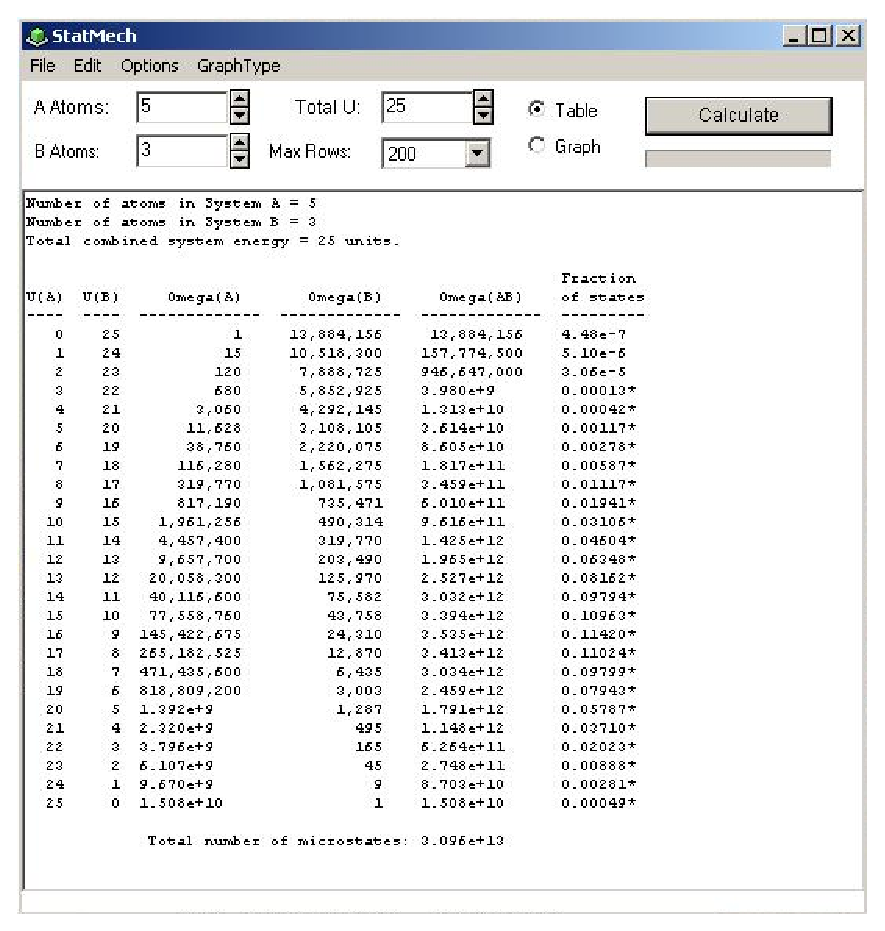
\includegraphics[height=4.0in]{S+T/statmech1.eps}
\caption{The {\tt StatMech} window showing the table of multiplicities for each microstate.
\index{color page}
Each row corresponds to a different value of $q_A$.}
\end{center}
\end{figure}
The first two columns in the lower panel of Figure 1 represent $U(A)$ and $U(B)$, 
the energies in each 
individual solid (again in units of $\hbar \omega$) and are equivalent to $q_A$ and $q_B$.
After you perform the calculation with {\it StatMech} scan quickly down the column
labeled `Omega(AB)'.
If any of the exponents you see exceed the value 307, then run the calculation again with 
smaller inputs until no exponent exceeds 307.
This limitation is a restriction on MicroSoft {\it Excel} that you will use later to make
plots.
Record your values of $N_A$, $N_B$, and $U$.
\vspace{15mm}

(b) Now generate plots of $S_{AB}=S_A + S_B$, $S_A$, and $S_B$ from the {\it StatMech} table.
You can do this with {\it Excel}, but there are some intermediate steps necessary.
Start Microsoft {\it Word} first.
Next, go to the {\it StatMech} window, highlight the table, copy it
 (see the {\tt Edit} menu on the {\it StatMech} window), and paste it into the {\it Word}
document. 
In {\it Word} edit out all the commas (`,') and asterisks (`*') in the file 
(use the {\tt Replace}
option under the {\tt Edit} menu).
Save the Word file, but save it as a plain text (`\*.txt') file.
You can now open the file in {\it Excel}.
When you open the file, {\it Excel} pops up a {\tt Text Import Wizard} 
that will guide you through
the format of the input file.
The defaults usually seem to work.
Use {\it Excel} to calculate and plot on one graph $S_{AB}$, $S_A$, and $S_B$
as a function of $q_A$.
Print out your plot and attach it to this unit.

(c) What is $q_A$ for the most probable macrostate? What mathematical condition can you impose
on the total entropy $S_{AB}$ to determine the most probable macrostate?
How do you think the temperatures of solids $A$ and $B$ are related at the most probable 
microstate?
\vspace{15mm}

(d) How are the slopes of $S_A$ and $S_B$ related to one another at the most probable
macrostate?
\vspace{30mm}

\newpage

(e) How is $E_A$, the energy in solid $A$ related to $q_A$?
How is $E_B$, the energy in solid $B$ related to $q_A$?
Remember that $q_{AB}$ is a constant and $q_{AB} = q_A + q_B$.
Calculate the differentials $dE_A$ and $dE_B$ and rewrite the answer in part 1.d
in terms of $dS_A/dE_A$ and $dS_B/dE_B$.
\vspace{45mm}

\textbf{Activity 2: Relating Entropy and Temperature}

(a) Using the spreadsheet you generated in Activity 1, calculate $dS_A/dq_A$ as a function
of $q_A$ and plot it. You can do this to an adequate approximation
by doing taking the difference between $S_A$ at adjacent values/rows
of $q_A$.
To do this suppose your spreadsheet has the values of $S_A$ in column $H$.
The {\it Excel} syntax for estimating the derivative for the first value of
$q_A$ (the first row) is 
`{\tt =(H2-H1)/1.0}' where {\tt H2} is the value in the second row and {\tt H1} is the
value in the first row.
The numerator of one is redundant, but it shows you are approximating the derivative
using the data from points that differ by 1.0 in $q_A$, the number of quanta in solid $A$.
The syntax for $dS_A/dq_A$ for the second value of $q_A$ is `{\tt =(H3-H2)/1.0}' and so on.
Do the same for $dS_B/dq_A$ and $dS_{AB}/dq_A$.
Does the slope of $S_{AB}$ pass through zero at the correct spot (recall part 1.c)?
How are $dS_A/dq_A$ and $dS_B/dq_A$ related at the most probable macrostate.
Does you plot agree with that result?
\vspace{15mm}

(b) If the energy $E_A$ and $q_A$ of solid $A$ increases what should the temperature 
of solid $A$ do?
If the energy $E_A$ of solid $A$ increases what happens to $dS_A/dq_A$ in your plot?
Do the temperature and $dS_A/dq_A$ change in the same  way or in a different way 
as $E_A$ increases?
\vspace{15mm}

(c) We want to come up with a relationship between temperature and the entropy.
From the results above (parts 1.a-e) you should have found
\begin{equation}
\frac{dS_A}{dE_A} = \frac{dS_B}{dE_B}
\end{equation}
and
\begin{equation}
T_A = T_B
\end{equation}
for the most probable macrostate.
This means there is some function of the temperature $T$ such that
\begin{equation}
f(T) = \frac{dS}{dE}
\end{equation}
for each solid that will be equal at equilibrium.
We want $f(T)$ to behave like the temperatures we are accustomed to using.
In other words, as the energy in the solid increases $T$ should increase.
Recall part 2.b and the behavior of $dS/dE$ as $T$ increases.
Try to guess a mathematical form of $f(T)$ that acts like `normal' temperatures
and one that doesn't. Explain your reasoning.
\vspace{30mm}

(d) How would you choose which of the forms you guessed in part 2.c is the correct one?
\vspace{15mm}

\textbf{Activity 3: Determining $f(T)$ and the Heat Capacity}

In the previous Activity you should have found that the mathematical form of $f(T)$
has to be something like $1/T^n$ where $n$ is some positive number.
This is necessary because your graphs should show that as the energy $E_A$ (and the number
of quanta $q_A$) of the solid 
increases $f(T)=dS/dE$ goes down. To make sure the temperature $T$ behaves reasonable
(and goes up with $E_A$ and $q_A$) $f(T)$ must be some inverse of function of $T$.
To decide exactly which function is right requires comparing Equation 7 or some
result from it to some data.

Recall the table of heat capacities we generated in the laboratory entitled
{\it Calorimetry}.
Use those results to fill in Table 1 making sure that you are using molar 
heat capacities.
\begin{table}
\begin{center}
\begin{tabular}{|p{0.8in}|l|p{0.8in}|l|} \hline
\hi Solid    & $dE/dT$ per mole & Solid      & $dE/dT$ per mole   \\[2pt] \hline
\hi          &                  &            &       \\[2pt] \hline
\hi          &                  &            &      \\[2pt] \hline
\hi          &                  &            &      \\[2pt] \hline
\end{tabular}
\caption{Molar specific heats ($(1/n)dE/dT$) for several elemental solids.}
\end{center}
\end{table}
%Consider Table 1 of heat capacities ($dE/dT$) for several elemental solids
%for high temperatures.
%\begin{table}
%\begin{center}
%\begin{tabular}{|p{0.8in}|l|p{0.8in}|l|} \hline
%\hi Solid    & $dE/dT$ per mole & Solid      & $dE/dT$ per mole   \\[2pt] \hline
%\hi Lead     & $26.4~J/K-mole$    & Gold     & $25.4~J/K-mole$      \\[2pt]
%\hi Silver   & $25.4~J/K-mole$    & Copper   & $24.5~J/K-mole$      \\[2pt]
%\hi Iron     & $25.0~J/K-mole$    & Aluminum & $26.4~J/K-mole$      \\[2pt] \hline
%\end{tabular}
%\caption{Heat capacities ($dE/dT$) for several elemental solids.}
%\end{center}
%\end{table}
 The heat capacities are constant with respect to temperature and are similar in value to
one another.
These are the data that will help us determine $f(T)$.
To calculate $dE/dT$ we must find a relationship between $E$ and $T$ for the Einstein solid.

(a) Start with Equations 1 and 7 and the chain rule and show the following.
\begin{equation}
\frac{dS}{dE} = k_B \frac{1}{\Omega} \frac{d\Omega}{dE}
\end{equation}
\vspace{15mm}

(b) Use Equation 2 to show 
\begin{equation}
dE = \hbar \omega dq \qquad {\rm and} \qquad  
    \frac{d\Omega}{dE}=\frac{1}{\hbar\omega} \frac{d\Omega}{dq}
\qquad .
\end{equation}
\vspace{15mm}

\newpage

(c) Starting with Equations 1 and 3 one can show
\begin{equation}
\frac{d\Omega}{dq} = \frac{3N\hbar \omega}{E} \Omega
\qquad .
\end{equation}
Combine this equation (number 10) and the  results from 3.a-b to 
get a relationship for $dS/dE$ for the Einstein solid in terms
of $N$ and $E$.
Set that expression equal to $f(T)$,
and solve for $E$ the internal energy.
It is the derivative of this last equation ($(1/n)dE/dT$) that will give you the molar specific heat.
What function of $f(T)$ will give a result that is independent of temperature when you
take the derivative with respect to $T$ of your expression for the internal energy $E$?
\vspace{45mm}

(d)  What is the final form of Equation 7 and $f(T)$?
\vspace{15mm}

(e) Determine the mean and standard deviation of the heat capacity of the elemental solids in
Table 1.
Calculate the molar specific heat ($(1/n)dE/dT$) for the Einstein solid using your results from
parts 3.c-d.
Is the molar specific heat for the model of the Einstein solid consistent with the measured ones?
\vspace{45mm}


\textbf{Activity 4: The Second Law of Thermodynamics}

(a) Go back to your plots of the entropy as a function of $q_A$ from part 1.b. 
Consider two Einstein solids that are brought together at a value of $q_A$ that is higher
than the equilibrium one at the most probable macrostate.
Choose a value of $q_A$ that is halfway between the most probable value and the maximum.
Once the two Einstein solids are in contact, how will the system evolve?
What happens to $S_A$ and $S_B$? Do they go up, down, or stay the same?
What happens to the total entropy $S_{AB}$?
In fact, based on your plot from part 2.b, is there any circumstance where
$S_{AB}$ will not increase?
\vspace{30mm}

(c) To  vividly see what happens when Einstein solids come in thermal contact,
run the program {\it equilib.exe} available in the {\tt Physics Applications} menu.
This program starts with two Einstein solids with all the energy quanta in solid $B$.
It simulates the evolution of the two solids as they march toward
thermal equilibrium.
Click {\tt Evolve} to see the simulation run.

What you should have discovered in the previous part is that the entropy of the combined systems
always increases regardless of what configuration the Einstein solids are in when they
come in contact.
The system always evolves to the most probable, most disordered
 macrostate where the temperatures will
be equal and the entropy is a maximum.
The energy quanta are most spread out.
This result is stated in several different ways, but the most succinct is simply
$\Delta S > 0$ for an isolated system.
The entropy of an isolated system always increases.
This is called the Second Law of Thermodynamics.

\bigskip

\textbf{Activity 4: Homework Problems}

\begin{enumerate}
 
\item (E) An object's entropy is measured to increase by $0.1~ J/K$ 
when we add $35~ J$ of energy.  What is its approximate temperature?  
(Assume that the object's temperature does not change much when we add the $35~J$.)

\item (E) A certain Einstein solid's entropy changes from 
$305.2k_b$ to $338.1k_b$ when we add 1 unit $\epsilon$ of energy.  
What is the value (and units) of $k_bT/\epsilon$ for this solid?  
If $\epsilon = 1.0~eV$, what is its temperature $T$?

\item (E) Does it make sense to talk about the 
temperature of a vacuum?  If so, how could you measure or calculate it?  
If not, why not?  

\item (E) An Einstein solid in a certain macrostate has a multiplicity of $3.8 \times 10^{280}$.  
What is its entropy (expressed as a multiple of $k_B$)?

\item (E) A pair of Einstein solids in a certain macropartition has multiplicities of 
$4.2 \times 10^{320}$ and $8.6 \times 10^{132}$.  What are the entropies of 
each solid?  What is the total 
entropy of the system in this macropartition?  (Express entropies as multiples of $k_b$.)

\item (E) Is it really true that the entropy of an isolated system consisting of two 
Einstein solids never decreases?  (Consider a pair of very small solids.)  Why is this 
statement more accurate for large systems than for small systems?  Explain in your own words.

\item (P) In lab we argued on fairly fundamental grounds 
that $dS/dU = f(T)$.  In principle, we could define $f(T)$ to be anything 
that we like:  this would amount to defining temperature and its scale. 
Still, some definitions would violate deeply embedded preconceptions 
about the nature of temperature.  
For example, the simplest definition of temperature would be $dS/dU = T_{new}$.  
Show that this definition
\begin{enumerate}
\item Would imply that $T_{new}$ has units of $K^{-1}$ and
\item Would imply that heat would flow spontaneously from objects with 
low $T_{new}$ to objects with high $T_{new}$.  
This would imply that object with low values of $T_{new}$ are hot, while 
objects with high values $T_{new}$ are cold (we might want to call $T_{new}$ 
so defined {\it coolness} instead of {\it temperature}).  
While we could define temperature in this way, it would really fly 
in the face of convention (if not intuition).
\item If we did define coolness $T_{new}$ in this way, what ordinary 
temperature $T$ would an object with absolutely zero coolness (
$T_{new} = 0$) have?  What about something that is infinitely cool ($T_{new} = \infty$)?
\end{enumerate}

\item (P) Imagine that the entropy of a certain substance as a function of 
$N$ and $U$ is given by the formula $S = Nk_b \ln U$. Using the definition of temperature, 
show that the thermal energy of this substance is related to its temperature 
by the expression $U=Nk_b T$.

\item (P) Imagine that the multiplicity of a certain substance is 
given by $\Omega(U,N) = Ne^{\sqrt{NU/\epsilon}}$, where $\epsilon$ is some unit of energy.  
How would the energy of an object made out of this substance depend 
on its temperature?  Would this be a `normal' substance in our usual sense 
of temperature.

\item (P) Consider an Einstein solid having $N = 20$ atoms.  
\begin{enumerate}
\item What is the solids temperature when it has an energy of $10\epsilon$, 
assuming that $\epsilon =h\omega = 0.02 eV$?  Calculate this directly from the 
definition of temperature by finding $S$ at $10\epsilon$ and $11\epsilon$, computing 
$dS/dU \approx [S(11\epsilon) - S(10\epsilon)]/\epsilon$, and then applying 
the definition of temperature.  (You will find that your work will 
go faster if you use {\it StatMech} to tabulate the multiplicities.)
\item How does this compare with the result from the formula $U = 3Nk_bT$ 
(which is only accurate if $N$ is large and $U/3N\epsilon > 1$)?
\item If you have access to {\it StatMech}, repeat for 
$N = 200$ and $U =100\epsilon$.  
(Hint:  If your calculator cannot handle numbers in excess of $10^{100}$, 
use the fact that in $(a \times 10^b) = \ln a + b \ln 10 $).
\end{enumerate}

\item (P)  A newly-created material has a multiplicity
$$
\Omega = \alpha N E
$$
where $N$ is the number of atoms in the solid,
$E$ is the total, internal energy in the solid, and $\alpha$ is a constant of 
proportionality.
\begin{enumerate}
\item How does the temperature of the new material depend on the internal energy?
\item What is the molar heat capacity for this solid?
\item Could this material really exist? Why or why not?
\end{enumerate}

\item (P)  A newly-created material has a multiplicity
$$
\Omega = \beta M E^2
$$
where $N$ is the number of atoms in the solid,
$E$ is the total, internal energy in the solid, and $\alpha$ is a constant of 
proportionality.
\begin{enumerate}
\item How does the temperature of the new material depend on the internal energy?
\item What is the molar heat capacity for this solid?
\item Could this material really exist? Why or why not?
\end{enumerate}


\end{enumerate}


